% !TEX root = ./0.main.tex

%In the industry, the sequential recommendation is a very demanding problem since, in e-commerce companies, we are facing users with long historical behaviors that rely on the predictions for recommendations. 
在本节中,我们将按顺序推荐进行实验,以评估我们框架与其他最新方法相比的性能。 此外,我们还将在十亿规模的工业数据集上报告我们框架的实验结果。

\begin{table}
  \centering
  \caption{\label{tab:match_stats} 数据集统计}
%   \renewcommand{\arraystretch}{1.2}
  \begin{tabular}{c|c|c|c}
    \hline \hline
    \textbf{Dataset} & \# users & \# items & \ \# interactions \\
    \hline
    Amazon Books & 459,133 & 313,966 & 8,898,041 \\
    % Amazon Electronics & 192,403 & 63001 & 1,689,188 \\
    % ML-20M & & & \\
    % Netflix & & & \\
    Taobao & 976,779 & 1,708,530 & 85,384,110 \\
    \hline \hline
  \end{tabular}
\end{table}

\begin{table*}[]
    \centering
    \caption{在公共数据集上的模型性能。 粗体数字是每一列的最佳性能。 表中所有数字均为百分号,省略了`\%'}
    % \renewcommand{\arraystretch}{1.2}
    \begin{tabular}{l|cccccc|cccccc}
        \hline \hline
        & \multicolumn{6}{c|}{Amazon Books} & \multicolumn{6}{c}{Taobao} \\
        & \multicolumn{3}{c}{Metrics@20} & \multicolumn{3}{c|}{Metrics@50} & \multicolumn{3}{c}{Metrics@20} & \multicolumn{3}{c}{Metrics@50} \\
        \hline
        & Recall & NDCG & Hit Rate & Recall & NDCG & Hit Rate & Recall & NDCG & Hit Rate & Recall & NDCG & Hit Rate \\
        \hline
        MostPopular & 1.368 & 2.259 & 3.020 & 2.400 & 3.936 & 5.226 & 0.395 & 2.065 & 5.424 & 0.735 & 3.603 & 9.309 \\
        YouTube DNN & 4.567 & 7.670 & 10.285 & 7.312 & 12.075 & 15.894 & 4.205 & 14.511 & 28.785 & 6.172 & 20.248 & 39.108 \\
        GRU4Rec & 4.057 & 6.803 & 8.945 & 6.501 & 10.369 & 13.666 & 5.884 & 22.095 & 35.745 & 8.494 & 29.396 & 46.068 \\
        % SASRec & & & & & & \\
        % Attention & 4.624 & 7.707 & 10.214 & 7.238 & 11.763 & 15.429 & & & & 2.496 & 29.808 & 47.845 \\
        MIND & 4.862 & 7.933 & 10.618 & 7.638 & 12.230 & 16.145 & 6.281 & 20.394 & 38.119 & 8.155 & 25.069 & 45.846 \\
        \hline
        \model-SA & \textbf{5.489} & 8.991 & 11.402 & \textbf{8.467} & \textbf{13.563} & 17.202 & \textbf{6.900} & \textbf{24.682} & 41.549 & 9.462 & 31.278 & 51.064 \\
        \model-DR & 5.311 & \textbf{9.185} & \textbf{12.005} & 8.106 & 13.520 & \textbf{17.583} & 6.890 & 24.007 & \textbf{41.746} & \textbf{9.818} & \textbf{31.365} & \textbf{52.418} \\
        \hline \hline
    \end{tabular}
    \label{tab:match_results}
\end{table*}

\subsection{实验准备}

% The matching stage plays a crucial role in recommendations due to the large-scale item pool of industrial recommender systems. 

我们在强泛化 ~\cite{marlin2004collaborative, liang2018variational, ma2019learning} 下评估所有方法的性能: 我们将所有用户按8:1:1的比例划分为训练/验证/测试集。我们使用训练用户的整个点击序列来训练模型。 为了进行评估,我们从验证和测试用户中提取用户行为的前80%,以通过预测剩余的20%用户行为,从经过训练的模型推断用户嵌入并计算指标。此设置比弱泛化要困难得多,在弱泛化中,在训练和评估过程中都使用用户的行为序列 ~\cite{liang2018variational}.
详细地说,我们采用训练顺序推荐模型的通用设置。 假设用户 $u$ 行为顺序为 $(e_1^{(u)}, e_2^{(u)}, ..., e_k^{(u)}, ..., e_n^{(u)})$。 每个训练样本都使用 $u$ 的前 $k$ 个行为来预测第 $(k+1)$ 个行为,其中 $k=1,2,...,(n-1)$。

\vpara{数据集.} 我们对两个具有挑战性的公共数据集进行了实验。 表~\ref{tab:match_stats}中显示了两个数据集的统计信息。

\begin{itemize}
    \item \textbf{Amazon}\footnote{\url{http://jmcauley.ucsd.edu/data/amazon/}} 由商品评论和来自亚马逊的元数据组成 ~\cite{mcauley2015image,he2016ups}. 在我们的实验中,我们使用Amazon数据集的 \textit{Books} 类别。 每个训练样本的长度为20。
    % \item \red{\textbf{MovieLens 20M}\footnote{https://grouplens.org/datasets/movielens/} consists of 20M movie ratings, which is a stable benchmark dataset. 20 million ratings and 465,000 tag applications are applied to 27,000 movies by 138,000 users. ML-20M includes tag genome data with 12 million relevance scores across 1,100 tags.}
    % \item \red{\textbf{Netflix}\footnote{http://www.netflixprize.com/} is user-movie rating data constructed to support participants in the Netflix Prize. The movie rating files contain over 100 million ratings from 480 thousand randomly-chosen, anonymous Netflix customers over 17 thousand movies. The data were collected between October, 1998 and December, 2005 and reflect the distribution of all ratings received during this period. The date of each rating and the title and year of release for each movie id are also provided.
    % }
    \item \textbf{Taobao}\footnote{\url{https://tianchi.aliyun.com/dataset/dataDetail?dataId=649\&userId=1}} 从淘宝的推荐系统中收集用户行为~\cite{zhu2018learning}。在我们的实验中,我们仅使用点击行为,并按时间对一个用户的行为进行排序。 每个训练样本的长度为50。
\end{itemize}
% For each user $u$, we sort the reviews from the user by time, and our task is to predict whether the user will write the review for the item based on previous reviews.
% Taobao dataset randomly selects about 1 million users who have behaviors including click, purchase, add-to-cart, and add-to-preference from November 25 to December 03, 2017. Each behavior is represented by five fields, which consist of user ID, item ID, item's category ID, behavior type, and timestamp.

\vpara{竞争者.} 我们将我们提出的模型,\model-SA 和 \model-DR 与目前最先进的模型比较。在我们的实验环境中,模型应该为验证和测试集的看不见的用户提供预测。 因此,基于分解的方法不适用于此设置。
\begin{itemize}
    \item \textbf{MostPopular} 是一种向用户推荐最受欢迎商品的传统推荐方法。
    % \item \textbf{Embedding\&MLP} is a basic deep learning model for CTR prediction formalized by~\cite{zhou2018deep, zhou2019deep}. The input features of items are first mapped into low dimensional embedding vectors and then transformed into fixed-length vectors using a pooling operator. 
    \item \textbf{YouTube DNN}~\cite{covington2016deep} 是工业推荐系统最成功的深度学习模型之一。
    \item \textbf{GRU4Rec}~\cite{hidasi2015session} 是为推荐引入RNN的第一篇著作。
    % It is worth mentioning that GRU4Rec can be used for either ranking task or matching task.
    % \item \textbf{ARNN} is a variation of GRU4Rec, which uses an attention mechanism to weighted sum over all the hidden states along time.
    % \item \textbf{RUM}~\cite{chen2018sequential} designs a memory-augmented neural network that integrated with the insights of collaborative filtering for the recommendation.
    % \item \textbf{SASRec}~\cite{kang2018self} captures long-term semantics by a self-attention based sequential model and makes predictions based on relatively few actions.
    \item \textbf{MIND}~\cite{li2019multi} 是与我们的模型相关的最新技术模型。 它基于胶囊路由机制设计了一个多兴趣提取器层,适用于聚类过去的行为并提取各种兴趣。
\end{itemize}

\vpara{实现说明.}
我们的实验代码使用了TensorFlow\footnote{\url{https://www.tensorflow.org/}} 1.14 在 Python 3.6下实现。 % The experiments on the two datasets are conducted using a single Linux server with 4 Intel(R) Xeon(R) CPU E5-2680 v4 @ 2.40GHz, 256G RAM, and 8 NVIDIA GeForce RTX 2080 Ti.
% The experiment is conducted using dozens of workers of Alibaba distributed cloud platform\footnote{https://data.aliyun.com/}. Every two workers share an NVIDIA Tesla P100 GPU with 16GB memory.

\vpara{参数配置.}
嵌入的维数 $d$ 设置为 64。采样的softmax损失的样本数设置为10。最大训练迭代次数设置为1百万。 多兴趣模型的兴趣嵌入数量设置为4。我们使用学习速度为 $lr=0.001$ 的 Adam 优化器 ~\cite{kingma2014adam} 进行优化。

% The batch size for the Amazon dataset and Taobao dataset is set to 128 and 256, respectively. The number of iterations for the dynamic routing method is set to 3.

\vpara{评估指标.}
我们使用以下指标来评估我们提出的模型的性能。 我们在实验中使用三种常用的评估标准。
\begin{itemize}
    \item \textbf{召回}. 为了更好地解释,我们采用每用户平均值而不是全局平均值,请参见~\cite{karypis2001evaluation,chen2018sequential}.
        \begin{equation}
            \operatorname{Recall@N} = \frac{1}{|\mathcal{U}|}\sum_{u\in \mathcal{U}} \frac{|\mathcal{\hat{I}}_{u,N} \cap \mathcal{I}_{u}|}{|\mathcal{I}_u|},
        \end{equation}
        其中 $\mathcal{\hat{I}}_{u,N}$ 表示用户 $u$ 的前N个推荐项的集合, $\mathcal{I}_u$ 是用户的测试项的集合 $u$.
    
    \item \textbf{命中率}. 命中率 (HR) 衡量推荐项目包含至少一个与用户互动的正确项目的百分比,该数据已在以前的工作中广泛使用~\cite{karypis2001evaluation,chen2018sequential}.
        \begin{equation}
            \operatorname{HR@N} = \frac{1}{|\mathcal{U}|}\sum_{u\in \mathcal{U}} \delta(|\mathcal{\hat{I}}_{u,N} \cap \mathcal{I}_{u}|>0),
        \end{equation}
        其中 $\delta(\cdot)$ 是指示函数

        % where $\mathcal{\hat{I}}_{u,N}$ denotes the set of top-$N$ recommendation items for user $u$ and $\mathcal{I}_u^{+}$ is the set of positive testing items for user $u$. $\delta(\cdot)$ is the indicator function.

    % \item \textbf{Mean Average Precision (MAP)}. There is only one target item per instance and thus the MAP@N increases with N which is consistent with ~\cite{belletti2018factorized,tang2019towards}.
    %     \begin{equation}
    %         \operatorname{MAP@N} = \frac{1}{|\mathcal{U}|}\sum_{u\in \mathcal{U}}  \frac{\sum_{k=1}^N P_u@k\times \delta(\hat{i}_{u,k}\in \mathcal{I}_u^{+})}{|\mathcal{\hat{I}}_{u,N}\cap \mathcal{I}_u^{+}|},
    %     \end{equation}
    %     \begin{equation}
    %         P_u@k = \frac{|\mathcal{\hat{I}}_{u,k}\cap \mathcal{I}_u^{+}|}{|\mathcal{\hat{I}}_{u,k}|},
    %     \end{equation}
    %     where $\mathcal{\hat{I}}_{u,N}$ denotes the set of top-$N$ recommendation items for user $u$, $\mathcal{I}_u^{+}$ is the set of positive testing items for user $u$, $\hat{i}_{u,k}$ denotes the $k$-th recommendation item, and $\delta(\cdot)$ denotes the indicator function. 


    \item \textbf{归一化折现累积收益}. 归一化折现累积收益 (NDCG) 考虑正确推荐项目的位置~\cite{jarvelin2000ir}.
        \begin{equation}
            \operatorname{NDCG@N} = \frac{1}{Z}\operatorname{DCG@N} = \frac{1}{Z} \frac{1}{|\mathcal{U}|}\sum_{u\in\mathcal{U}}\sum_{k=1}^{N}\frac{\delta(\hat{i}_{u,k}\in \mathcal{I}_{u})}{\operatorname{log}_2(k+1)},
        \end{equation}
        其中 $\hat{i}_{u,k}$ 表示用户 $u$ 的第 $k$ 个推荐项目, $Z$ 是一个标准化常数,表示理想的折现累积收益 (IDCG@N), 这是 DCG@N 的最大可能值。 
\end{itemize}

% \begin{figure*}
%     \centering
%     \includegraphics[width=0.9\textwidth]{figures/heatmap.pdf}
%     \caption{The heatmap of a user's four interests and the behavior sequence from the Amazon dataset. From the heatmap, we can see that our model learns four different interests from the behavior sequence. The 0th, 1st, 2nd, and 3rd interests are related to the ``Health'', ``Business'', ``Cookbooks'', and ``Self-Help'' categories, respectively. Our model learns the category information from the user sequence, although only item IDs are used for model training.}
%     \label{fig:case_study_heatmap}
% \end{figure*}


% \begin{table*}[]
%     \centering
%     \caption{Book titles and categories of the user behavior sequence from the Amazon dataset.}
%     \begin{tabular}{c|l|l}
%         \hline \hline
%         No. & Book Title & Category \\
%         \hline
%         0 & MAKE MONEY ONLINE ON ELANCE & Business \& Money \\
%         1 & Cure Acne Overnight & Health, Fitness \& Dieting \\
%         2 & Headling Your Inner Child & Self-Help \\
%         3 & SOCIAL MEDIA MARKETING FOR BEGINNERS & Business \& Money \\
%         4 & POSITIVE THINKING: The Ultimate Guide To Mastering Positive Thinking & Self-Help \\
%         5 & COMMUNICATION SKILLS Secrets & Self-Help \\
%         6 & THE MEDITERRANEAN DIET ROCKS!!! & Cookbooks, Food \& Wine \\
%         7 & REAL ESTATE WHOLESALING REVEALED & Business \& Money \\
%         8 & HOW TO GET CUSTOMERS IN YOUR NETWORK MARKETING COMPANY & Business \& Money \\
%         9 & THE PALEO COMFORT FOODS COOKBOOK & Cookbooks, Food \& Wine \\
%         10 & CREATIVITY: Discover How To Unlock Your Creative Genius And Release The Power Within & Health, Fitness \& Dieting \\
%         11 & GREEK CUISINE COOKBOOK & Cookbooks, Food \& Wine \\
%         12 & Gluten-Free Vegan Cookbook & Cookbooks, Food \& Wine \\
%         \hline \hline
%     \end{tabular}
%     \label{tab:case_study_cate}
% \end{table*}

\subsection{定量结果}
% \subsection{Performance Analysis.}
为了与其他模型进行公平比较,我们在聚合模块中设置 $\lambda=0$ 。我们将详细介绍如何检索框架的前N个项目。 对于我们的框架,用户的每个兴趣都独立检索前N个候选项目。 因此,我们的模型为每个用户检索了总计 $K\cdot N$ 个项目。 我们通过项目嵌入的内积和相应的兴趣嵌入对项目进行排序。 排序之后,这些 $K\cdot N$ 个项目中的前N个项目被视为模型的最终候选项目。 检索候选项目的方法也适用于MIND。
表~\ref{tab:match_results}中显示了顺序推荐的模型性能。在所有评估标准上,我们的模型均优于所有最新模型。 与仅为每个用户输出单个嵌入的其他模型相比,GRU4Rec可获得最佳性能。 与MIND相比 \model-DR 由于动态路由方法的差异而获得了更好的性能。 \model-SA 自注意力机制显示出强大的捕获用户兴趣的能力,并且可以与 \model-DR 取得可比的结果。
% The performance shows that our model has a strong ability to capture user interests. 
%With the penalty term, multiple interests of users can be better disentangled and the performance improves. 


% \begin{figure}[t]
%     \centering
% %     \subfigure[Interest Number]{\includegraphics[width=0.23\textwidth]{figures/interest_num.png}}
% %  	\subfigure[Iteration Number]{\includegraphics[width=0.23\textwidth]{figures/iteration_num.png}}
%     \includegraphics[width=0.50\textwidth]{figures/sensitivity.pdf}
% 	\caption{Model performance w.r.t. the number of user interests and the iteration of the dynamic routing method}
%     \label{fig:ctr_sensitivity}
% \end{figure}

\begin{table}
  \centering
  \caption{\label{tab:match_ps} 参数灵敏度的模型性能。 所有数字均为百分比数字,省略了 `\%' }
%   \renewcommand{\arraystretch}{1.2}
  \begin{tabular}{l|cc|cc}
    \hline \hline
    & \multicolumn{2}{c|}{Amazon Books} & \multicolumn{2}{c}{Taobao} \\
    Metric@50 & Recall & NDCG & Recall & NDCG \\
    \hline
    \model-SA (K=2) & 8.835 & \textbf{14.273} & 9.935 & 32.873 \\
    \model-SA (K=4) & 8.467 & 13.563 & 9.462 & 31.278 \\
    \model-SA (K=6) & \textbf{8.901} & 14.167 & 9.378 & 31.020 \\
    \model-SA (K=8) & 8.547 & 13.631 & 9.493 & 31.196 \\
    \hline
    \model-DR (K=2) & 7.081 & 12.068 & 9.293 & 30.735 \\
    \model-DR (K=4) & 8.106 & 13.520 & 9.818 & 31.365 \\
    \model-DR (K=6) & 7.904 & 13.219 & 10.836 & \textbf{34.048} \\
    \model-DR (K=8) & 7.760 & 12.900 & \textbf{10.841} & 33.895 \\
    \hline \hline
  \end{tabular}
\end{table}

\vpara{参数灵敏度.}
我们研究了我们框架的兴趣数量 $K$ 的灵敏读。表格~\ref{tab:match_ps}说明了超参数 $K$ 更改时我们框架的性能。 我们的两个模型显示了此超参数的不同属性。 对于Amazon数据集,当 $K=2, 6$ 时,\model-SA 获得更好的性能,而在 $K=4$ 时,\model-DR 获得最佳结果。 对于淘宝数据集,当 $K$ 从2增加到8时,\model-DR 获得更好的性能,但是当 $K=2$ 时,\model-SA 获得最佳结果。

\begin{table}
  \centering
  \caption{\label{tab:control} 可控制研究的Amazon数据集的模型性能。 所有数字均为百分比数字,省略了 `\%' }
%   \renewcommand{\arraystretch}{1.2}
  \begin{tabular}{c|cc|cc}
    \hline \hline
    & \multicolumn{2}{c|}{\model-SA (K=4)} & \multicolumn{2}{c}{\model-DR (K=4)} \\
    Metric@50 & Recall & Diversity & Recall & Diversity \\
    \hline
    $\lambda=0.00$ & \textbf{8.467} & 23.237 & \textbf{8.106} & 19.036 \\
    $\lambda=0.05$ & 8.347 & 38.808 & 7.931 & 42.915 \\
    $\lambda=0.10$ & 8.229 & 46.731 & 7.850 & 46.258 \\
    $\lambda=0.15$ & 8.142 & 51.135 & 7.820 & 46.912 \\
    $\lambda=0.20$ & 8.086 & 53.671 & 7.783 & 47.581 \\
    $\lambda=0.25$ & 8.034 & \textbf{55.100} & 7.764 & \textbf{48.375} \\
    \hline \hline
  \end{tabular}
\end{table}

\subsection{可控性研究}
\label{sec:control_study}
% Our proposed model generates multiple embeddings for each user. 
%A straightforward method is to sort the items based on their scores. However, each interest of a user is not equally important.
为了获得每个用户的最终前N个候选项目,我们提出了一个新颖的模块来汇总每个用户的不同兴趣所检索的项目。
除了要达到较高的推荐预测准确度外,一些研究还建议需要多样化的推荐,以避免单调并改善客户体验~\cite{gogna2017balancing,cheng2017learning}. 

在当前推荐系统中,推荐多样性起着更重要的作用。 许多研究旨在提高推荐的多样性,例如~\cite{bradley2001improving,qin2013promoting}。 我们提出的汇总模块可以控制推荐准确性和多样性之间的平衡。 我们根据项目类别使用以下个体多样性的定义:
\begin{equation}
    \operatorname{Diversity@N} = \frac{\sum_{j=1}^N \sum_{k=j+1}^N \delta(\operatorname{CATE}(\hat{i}_{u,j}) \neq \operatorname{CATE}(\hat{i}_{u,k}))}{N \times (N-1) / 2},
\end{equation}
\noindent 其中 $\operatorname{CATE}(i)$ 时物品 $i$ 的类别, $\hat{i}_{u,j}$ 表示用户 $u$ 的第 $j$ 个推荐项目,并且 $\delta(\cdot)$ 是一个指示函数. 

表~\ref{tab:control} 显示了当我们控制因素 $\lambda$ 以平衡推荐质量和多样性时,Amazon数据集的模型性能。 从表中可以看出,当可控因素 $\lambda$ 增加时,推荐多样性会大大增加,而召回率则略有下降。 通过为超参数 $\lambda$ 选择合适的值,我们的聚合模块可以在精度和多样性之间实现最佳平衡。


% \vpara{Ablation Study.}


% \begin{itemize}
%     \item \textbf{Precision, Recall, and F1-score}. We adopt the global average of all the users as follows. 
%         \begin{equation}
%             \operatorname{Precision} = \frac{\sum_{u\in \mathcal{U}}\sum_{i\in \mathcal{I}_u^{+}}\delta(\hat{y}_{ui}=1)}{\sum_{u\in \mathcal{U}}\sum_{i\in \mathcal{I}_u^{+} \cup \mathcal{I}_u^{-}}\delta(\hat{y}_{ui}=1)},
%         \end{equation}
%         \begin{equation}
%             \operatorname{Recall} = \frac{\sum_{u\in \mathcal{U}}\sum_{i\in \mathcal{I}_u^{+}}\delta(\hat{y}_{ui}=1)}{\sum_{u\in \mathcal{U}}|\mathcal{I}_u^{+}|},
%         \end{equation}
%         \begin{equation}
%             \operatorname{F1} = \frac{2\cdot \operatorname{Precision} \cdot \operatorname{Recall}}{\operatorname{Precision} + \operatorname{Recall}},
%         \end{equation}
%         where $\mathcal{I}_u^{+/-}$ is the set of positive/negative testing items, $\hat{y}_{ui}$ is the prediction of user $u$ interacting with item $i$, and $\delta(\cdot)$ is the indicator function. 
%     \item \textbf{AUC}. AUC is one of the most important evaluation metrics for measuring the performance of classification model.
%         \begin{equation}
%         \operatorname{AUC} =  \frac{1}{|\mathcal{D}^{+}||\mathcal{D}^{-}|} \sum_{(u,j)\in \mathcal{D}^{+}} \sum_{(v,k)\in \mathcal{D}^{-}} \delta(\hat{p}_{u,j} > \hat{p}_{v,k}),
%         \end{equation}
%         where $\mathcal{D}^{+/-}$ is the set of positive/negative training samples, $\hat{p}_{u,j}$ is the predicted probability, and $\delta(\cdot)$ is the indicator function. 
% \end{itemize}


% \vpara{Performance Analysis.}
% The experimental results for the ranking task are shown in Table~\ref{tab:rank_results}. The mean with the standard error of AUC and F1-score is reported. All figures are trained for 10 times with random seed from 1 to 10. For the Amazon dataset, our model performs as well as MIMN and surpasses other models significantly. Our model takes much less time than MIMN for training as MIMN uses complicated architecture based on memory networks. For the Taobao dataset, our model outperforms all state-of-the-art models by a wide margin. The performance shows that our model has a strong ability to capture long-term and short-term user interests. % With the penalty term, multiple interests of users can be better disentangled and the performance improves on Taobao dataset. 


% \vpara{Ablation Study.}
% To show how each encoder contributes to the overall performance, we present the ablation study on our ranking model. We use T, S, L to denote the tiny-term, short-term, and long-term encoders, respectively. Our multi-interest capsule network can be viewed as a long-term encoder. We report the performance of our model using a different configuration of encoders as Table~\ref{tab:ctr_ablation} shows. In the Amazon dataset, our long-term encoder is a crucial part of the overall model. In the Taobao dataset, the combination of the tiny-term and short-term encoders obtains the best performance. The result shows that different encoders play different roles in the ranking task on different datasets. The difference between the two datasets may be caused by different types of behaviors. The Amazon dataset collects user review sequences, and the Taobao dataset collects user click sequences. The click behaviors rely more on tiny-term and short-term behaviors than review behaviors. From the ablation study, we can also see that mixture models obtain better performance than the single model. It is consistent with our motivation that a single model has limitations, and a mixture model is needed for the ranking stage of recommender systems. 


\subsection{工业应用结果}

\begin{table}
  \centering
  \caption{\label{tab:industrial_stats} 工业数据集的统计}
%   \renewcommand{\arraystretch}{1.2}
  \begin{tabular}{c|c|c|c}
    \hline \hline
    \textbf{Dataset} & \# users & \# items & \# interactions \\
    \hline
    Industrial & 145,606,322 & 22,554,170 & 4,322,505,616 \\
    \hline \hline
  \end{tabular}
\end{table}


% \begin{figure}
%     \centering
%     \includegraphics[width=0.48\textwidth]{figures/tmp_picture.pdf}
%     \caption{The architecture of Taobao's recommender system.}
%     \label{fig:taobao_rs}
% \end{figure}

% The architecture of Taobao's recommender system is described as Figure~\ref{fig:taobao_rs}.

我们对2020年2月8日通过Mobile Taobao App收集的工业数据集进行了进一步的实验。工业数据集的统计信息显示在表格~\ref{tab:industrial_stats}中。工业数据集包含2200万个高质量项目,1.45亿用户以及它们之间的40亿行为。%\footnote{https://data.aliyun.com/}

我们的框架已部署在阿里巴巴分布式云平台上,其中每两个工作人员共享一个具有16GB内存的NVIDIA Tesla P100 GPU。 我们划分用户并使用训练用户的点击序列来训练我们的模型。 为了进行评估,我们使用模型为测试集中的每个用户计算多个兴趣。 用户的每个兴趣向量通过快速最近邻居方法独立地从大型项目池中检索前N个项目。 不同用户兴趣所检索的项目将被馈送到我们的汇总模块中。 在此模块之后, $K\cdot N$ 个项目中的前N个项目是最终的候选项目,并用于计算评估指标:retret @ 50。

我们在我们的框架和最新的顺序推荐方法~\cite{li2019multi}之间进行了离线实验,该方法已证明阿里巴巴集团的推荐系统得到了重大改进。 实验结果表明,与MIND相比,我们的\ model-SA和\ model-DR分别将召回率@ 50提高了1.39%和8.65%。

\begin{figure}
    \centering
    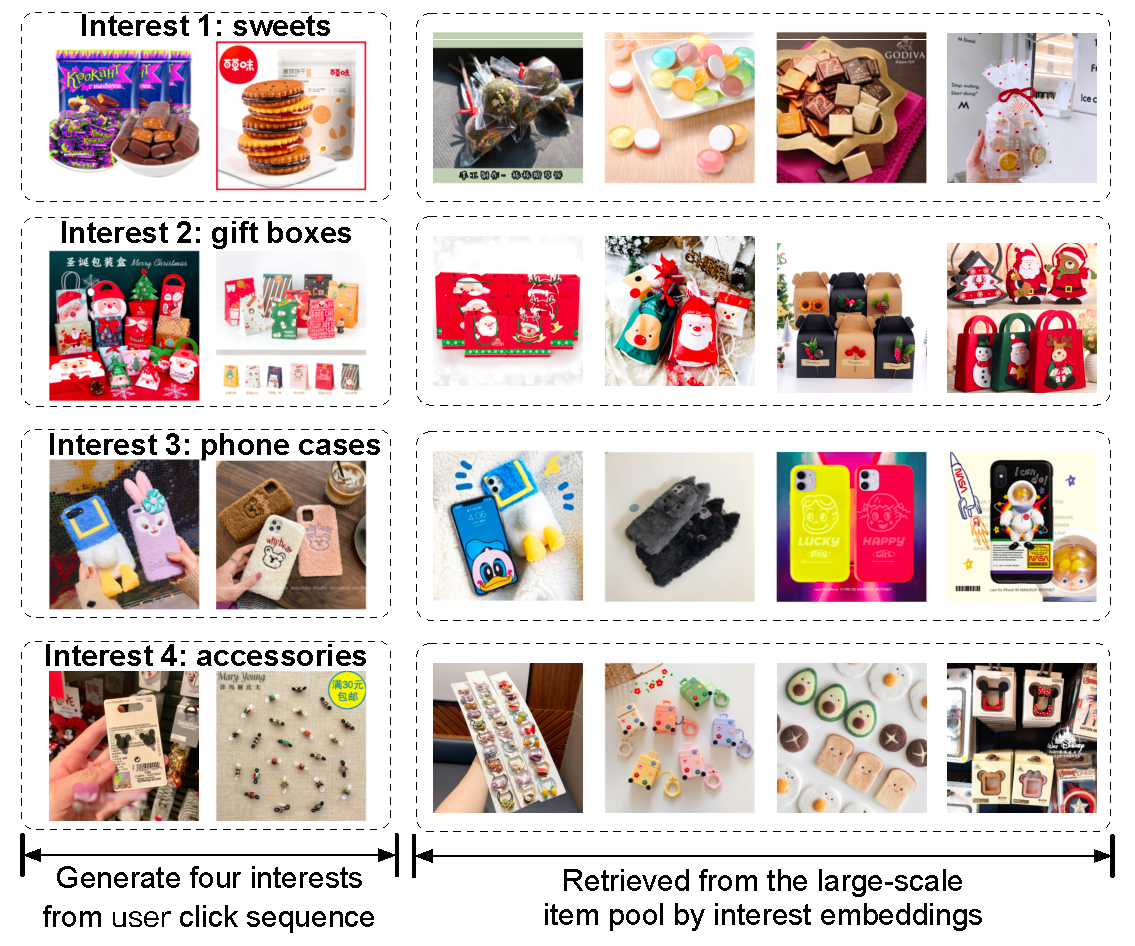
\includegraphics[width=0.47\textwidth]{figures/case_study.pdf}
    \caption{电子商务用户的案例研究。 我们的模型根据用户的点击顺序生成了四个兴趣嵌入。 我们发现用户的四个兴趣是关于糖果,礼品盒,电话盒和配件。 我们按点击顺序报告与这四个兴趣相对应的那些项目。 右侧部分显示了通过兴趣嵌入从工业项目库中检索到的项目。}
    \label{fig:case_study_interests}
\end{figure}


\vpara{案例分析.}
从图~\ref{fig:case_study_interests},我们可以看到我们的模型从用户的点击顺序中学习了用户的四种不同兴趣。 值得注意的是,我们的模型仅使用项目ID进行训练,而不使用人工定义的项目类别信息。 尽管如此,我们的模型仍然可以从用户行为序列中学习商品类别。 我们的模型学习到的每个兴趣大约对应一个特定类别,并且可以从大型工业项目池中检索相同类别的相似项目。


% The experimental goal is to maximize hit rate@N. We conduct an offline test on our matching model and xx. The results demonstrate that our model improves the hit rate by xx\% compared to xx.
